\section{Overførelsesfunktion af pendulet}\label{sec:sec_penduloverforelse}
Ved at Laplace-transformere ligningen \ref{eq:system_final}, findes $\theta(s)$
\begin{align}
 m_vLs^2\theta(s) - mg = -m_pL\theta(s) -mA_v(s) \\
 \theta(s)\left(m_vLs^2 - mg \right) = -m_pL\theta(s) -mA_v(s) \\
 \theta(s) = \frac{1}{m_vLs^2 - mg }\left[-m_pL\theta(s) -mA_v(s)\right] \label{eq:pendul_final}
\end{align} 
 
Ved at opstille overførelsesfunktionen i ligning \ref{eq:pendul_final} som model i figur \ref{fig:pendul_trans1}, fremgår de ind- og udgående variabler tydeligt. 

\begin{figure}[h!]
	\centering
	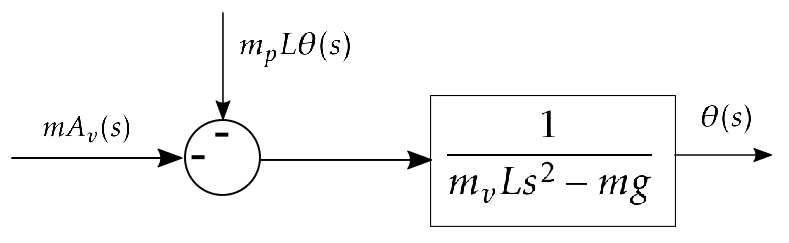
\includegraphics[width=.6\textwidth]{billeder/pendul_trans1.png}
	\caption[Model af overførelsesfunktion for vogn og pendul.]{Model af overførelsesfunktion for vogn og pendul fra ligning \ref{eq:pendul_final}.}
	\label{fig:pendul_trans1}
\end{figure}
\FloatBlock

I overførelsesfunktionen for pendulet indgår massen for vognen $m_v$ og den samlede masse for systemet $m = m_v + m_p$.
Da det ønskes at forsimple pendulets overførelsesfunktion antagess der, at massen af pendulet er lille i forhold til massen af vognen. 
Der kan således laves approksimationen $m \approx m_v$ og der fås således
\begin{align}
\frac{1}{m_vLs^2 - mg } \approx  \frac{1}{m \left( Ls^2 - g \right) } 
\end{align}
Modellen i figur \ref{fig:pendul_trans1} kan nu forenkles yderligere, hvorved masserne næsten udgår af systemet.
Den eneste tilbageblivende masse, er for forstyrrelsen på pendulstangen, der ender som $m_pL\theta(s) \approx  \frac{m_p}{m_v}L\theta(s) $.

\begin{figure}[h!]
	\centering
	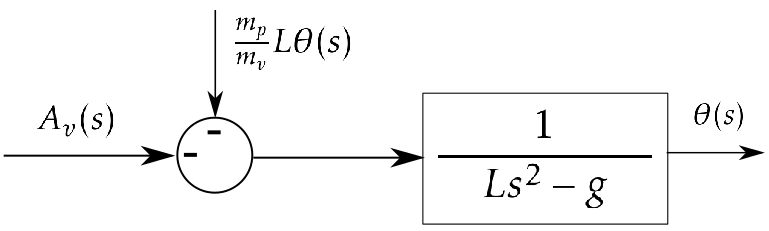
\includegraphics[width=.6\textwidth]{billeder/pendul_trans_clean.png}
	\caption{Simplificeret model af overførelsesfunktion for vogn og pendul.}
	\label{fig:pendul_trans_clean}
\end{figure}
\FloatBlock 
Således fås en model (figur \ref{fig:pendul_trans_clean}) af pendulet, der relaterer en påført acceleration $A_v(s)$ til en ændring af vinklen $\theta(s)$
